
%(BEGIN_QUESTION)
% Copyright 2010, Tony R. Kuphaldt, released under the Creative Commons Attribution License (v 1.0)
% This means you may do almost anything with this work of mine, so long as you give me proper credit

A thermal mass flowmeter uses two RTD sensing elements (one heated, one unheated) to infer mass flow rate through a pipe.  The following circuit converts the difference in RTD temperatures into a voltage signal for a microprocessor to interpret:

$$\includegraphics[width=15.5cm]{i02946x01.eps}$$

A {\it current mirror} works to keep current through both RTDs equal, while a differential amplifier measures the difference in voltage drops across the two RTDs.

\vskip 10pt

Unfortunately, this flowmeter is not functioning as it should.  The microprocessor reports an over-ranged flow measurement even when the flowmeter has been ``blocked in'' by closing block valves both upstream and downstream in the pipe.  You are summoned to troubleshoot this circuit, and you begin by measuring the output voltage from the amplifier -- you read 0 volts DC with your voltmeter.  Next, you measure voltage between test points {\bf C} and {\bf B}, again measuring 0 volts DC.

Identify the likelihood of each specified fault for this circuit.  Consider each fault one at a time (i.e. no coincidental faults), determining whether or not each fault could independently account for {\it all} measurements and symptoms in this circuit.

% No blank lines allowed between lines of an \halign structure!
% I use comments (%) instead, so that TeX doesn't choke.

$$\vbox{\offinterlineskip
\halign{\strut
\vrule \quad\hfil # \ \hfil & 
\vrule \quad\hfil # \ \hfil & 
\vrule \quad\hfil # \ \hfil \vrule \cr
\noalign{\hrule}
%
% First row
{\bf Fault} & {\bf Possible} & {\bf Impossible} \cr
%
\noalign{\hrule}
%
% Another row
22 k$\Omega$ resistor failed open &  &  \cr
%
\noalign{\hrule}
%
% Another row
Unheated RTD failed open &  &  \cr
%
\noalign{\hrule}
%
% Another row
Heated RTD failed open &  &  \cr
%
\noalign{\hrule}
%
% Another row
Unheated RTD failed shorted &  &  \cr
%
\noalign{\hrule}
%
% Another row
Heated RTD failed shorted &  &  \cr
%
\noalign{\hrule}
%
% Another row
Transistor Q$_1$ failed shorted C-E &  &  \cr
%
\noalign{\hrule}
%
% Another row
Transistor Q$_2$ failed shorted C-E &  &  \cr
%
\noalign{\hrule}
%
% Another row
12 VDC source dead &  &  \cr
%
\noalign{\hrule}
} % End of \halign 
}$$ % End of \vbox

Also, explain why these initial voltage measurements made sense to take.  In other words, explain what each measurement told you about the nature of the fault.  

Finally, identify the {\it next} diagnostic test or measurement you would make on this system.  Explain how the result(s) of this next test or measurement help further identify the location and/or nature of the fault.

\underbar{file i02946}
%(END_QUESTION)





%(BEGIN_ANSWER)


%(END_ANSWER)





%(BEGIN_NOTES)

% No blank lines allowed between lines of an \halign structure!
% I use comments (%) instead, so that TeX doesn't choke.

$$\vbox{\offinterlineskip
\halign{\strut
\vrule \quad\hfil # \ \hfil & 
\vrule \quad\hfil # \ \hfil & 
\vrule \quad\hfil # \ \hfil \vrule \cr
\noalign{\hrule}
%
% First row
{\bf Fault} & {\bf Possible} & {\bf Impossible} \cr
%
\noalign{\hrule}
%
% Another row
22 k$\Omega$ resistor failed open & $\surd$ &  \cr
%
\noalign{\hrule}
%
% Another row
Unheated RTD failed open &  & $\surd$ \cr
%
\noalign{\hrule}
%
% Another row
Heated RTD failed open &  & $\surd$ \cr
%
\noalign{\hrule}
%
% Another row
Unheated RTD failed shorted &  & $\surd$ \cr
%
\noalign{\hrule}
%
% Another row
Heated RTD failed shorted &  & $\surd$ \cr
%
\noalign{\hrule}
%
% Another row
Transistor Q$_1$ failed shorted C-E &  & $\surd$ \cr
%
\noalign{\hrule}
%
% Another row
Transistor Q$_2$ failed shorted C-E &  & $\surd$ \cr
%
\noalign{\hrule}
%
% Another row
12 VDC source dead & $\surd$ &  \cr
%
\noalign{\hrule}
} % End of \halign 
}$$ % End of \vbox

The 0 VDC measurement at the amplifier's output told you the microprocessor was correctly interpreting the signal, as 0 volts {\it should} cause it to register over-ranged flow.  This is true since only under infinite flow conditions should both the heated and unheated RTDs be at the same temperature!

The next measurement between test points {\bf C} and {\bf B} is to see what signal the amplifier is getting from the RTDs.  In other words, we're checking to see whether or not the amplifier has any differential signal to amplify.  If so, we know the amplifier has a problem.  If not (as is the case here), we know there is a problem somewhere in the current mirror / RTD network because we {\it do} expect to read a voltage here.

\vskip 20pt \vbox{\hrule \hbox{\strut \vrule{} {\bf Virtual Troubleshooting} \vrule} \hrule}

This question is a good candidate for a ``Virtual Troubleshooting'' exercise.  Presenting the diagram to students, you first imagine in your own mind a particular fault in the system.  Then, you present one or more symptoms of that fault (something noticeable by an operator or other user of the system).  Students then propose various diagnostic tests to perform on this system to identify the nature and location of the fault, as though they were technicians trying to troubleshoot the problem.  Your job is to tell them what the result(s) would be for each of the proposed diagnostic tests, documenting those results where all the students can see.

During and after the exercise, it is good to ask students follow-up questions such as:

\begin{itemize}
\item{} What does the result of the last diagnostic test tell you about the fault?
\item{} Suppose the results of the last diagnostic test were different.  What then would that result tell you about the fault?
\item{} Is the last diagnostic test the best one we could do?
\item{} What would be the ideal order of tests, to diagnose the problem in as few steps as possible?
\end{itemize}

%INDEX% Measurement, flow: thermal (mass)
%INDEX% Troubleshooting review: electric circuits

%(END_NOTES)

